\section{Merge}
\subsection{Introducción}
\textit{Merge} es un procedimiento en el cual se mezclan dos imágenes. Se reciben como inputs las imágenes a mergear, y luego se realiza un promedio ponderado (a partir de un valor recibido por parámetro) entre los píxeles de ambas imágenes, generando como salida una imagen que contiene el merge de las mismas.\\
La fórmula a partir de la cual se procesan los píxeles de las imágenes a mergear, sean estas A y B y donde value es el valor pasado por parámetro es:  

\begin{verbatim}
         A[j][i][k] = value * A[j][i][k] + (1-value) * B[j][i][k];
\end{verbatim}

Donde \textit{k} itera sobre las componentes del pixel, dejando inalterada la componente de transparencia.

\subsection{Pseudocódigo en C}

El pseudocódigo para una iteración del ciclo de la implementación que recibimos por parte de la cátedra es:

\begin{lstlisting}
// sean A y B las dos imagenes pasadas por parametro y value un float recibido tambien como input.
  for(ih=0;ih<(int)h;ih++) {		//itero sobre la altura de la imagen
   for(iw=0;iw<(int)w;iw++) {		//itero sobre el ancho de la imagen
    for(ii=1;ii<4;ii++) {			  //itero sobre los cuatro componentes RGBA del pixel
     A[ih][iw][ii] = (value*(A[ih][iw][ii]) + (1.0-value)*(B[ih][iw][ii])); //proceso dicha componente de pixel.
      }
    }
  }

\end{lstlisting}

De esta manera, lo que se hace es iterar por cada pixel de cada imagen y por cada una de sus componentes, realizando el cálculo correspondiente y guardando el resultado en una de las imágenes recibidas como input.

\subsection{Implementación 1 en ASM}
La primera implementación requiere realizar operaciones en punto flotante y procesar la mayor cantidad de pixeles posibles por iteración.\\
Como cada pixel mide 4B (1B por cada componente), en un registro XMM es posible procesar de a 4 a la vez. De esta forma, en cada iteración del ciclo tomamos 4 pixeles de cada imagen.

El procedimiento entonces será:

\begin{enumerate}
\item Tomar 4 pixeles de cada imagen.

\begin{tabular}{| o | o | o | o |} %tabla color orange
\hline
$Pa_{3}$ & $Pa_{2}$ & $Pa_{1}$ & $Pa_{0}$ \\ 
\hline
\end{tabular}

\begin{tabular}{| g | g | g | g |} %tabla color verde
\hline
$Pb_{3}$ & $Pb_{2}$ & $Pb_{1}$ & $Pb_{0}$ \\
\hline
\end{tabular}

$Pa_{i}$ y $Pb_{i}$ son los pixeles íesimos de las imagenes A y B.\\

\item Desempaquetar de byte a word y de word a dword.

\begin{tabular}{| o | o | o | o | o | o | o | o | o | o | o | o | o | o | o | o |} %tabla color orange
\hline
$0$ & $Pa_{3a}$ & $0$ & $Pa_{3b}$ & $0$ & $Pa_{3c}$ & $0$ & $Pa_{3d}$ & $0$ & $Pa_{2a}$ & $0$ & $Pa_{2b}$ & $0$ & $Pa_{2c}$ & $0$ & $Pa_{2d}$ \\ 
\hline
\end{tabular}

\begin{tabular}{| o | o | o | o | o | o | o | o | o | o | o | o | o | o | o | o |} %tabla color orange
\hline
$0$ & $Pa_{1a}$ & $0$ & $Pa_{1b}$ & $0$ & $Pa_{1c}$ & $0$ & $Pa_{1d}$ & $0$ & $Pa_{0a}$ & $0$ & $Pa_{0b}$ & $0$ & $Pa_{0c}$ & $0$ & $Pa_{0d}$ \\ 
\hline
\end{tabular}

En los dos registros anteriores quedan expresados las componentes de los 4 primeros píxeles tras ser desempaquetados de byte a word.

\begin{tabular}{| o | o | o | o | o | o | o | o | o | o | o | o | o | o | o | o |} %tabla color orange
\hline
$0$ & $0$ & $0$ & $Pa_{3a}$ & $0$ & $0$ & $0$ & $Pa_{3b}$ & $0$ & $0$ & $0$ & $Pa_{3c}$ & $0$ & $0$ & $0$ & $Pa_{3d}$ \\ 
\hline
\end{tabular}

\begin{tabular}{| o | o | o | o | o | o | o | o | o | o | o | o | o | o | o | o |} %tabla color orange
\hline
$0$ & $0$ & $0$ & $Pa_{2a}$ & $0$ & $0$ & $0$ & $Pa_{2b}$ & $0$ & $0$ & $0$ & $Pa_{2c}$ & $0$ & $0$ & $0$ & $Pa_{2d}$ \\ 
\hline
\end{tabular}

\begin{tabular}{| o | o | o | o | o | o | o | o | o | o | o | o | o | o | o | o |} %tabla color orange
\hline
$0$ & $0$ & $0$ & $Pa_{1a}$ & $0$ & $0$ & $0$ & $Pa_{1b}$ & $0$ & $0$ & $0$ & $Pa_{1c}$ & $0$ & $0$ & $0$ & $Pa_{1d}$\\ 
\hline
\end{tabular}

\begin{tabular}{| o | o | o | o | o | o | o | o | o | o | o | o | o | o | o | o |} %tabla color orange
\hline
$0$ & $0$ & $0$ & $Pa_{0a}$ & $0$ & $0$ & $0$ & $Pa_{0b}$ & $0$ & $0$ & $0$ & $Pa_{0c}$ & $0$ & $0$ & $0$ & $Pa_{0d}$ \\ 
\hline
\end{tabular}

En estos últimos cuatro registros, quedan expresados en words las componentes de los 4 píxeles, donde $Pa_{ij}$ representa al pixel iésimo de la imagen A en su componente j, y j puede ser R,G,B o A.

Análogamente, se realiza el desempaquetado para los píxeles de la imagen B. 

Primero de byte a word.

\begin{tabular}{| g | g | g | g | g | g | g | g | g | g | g | g | g | g | g | g |} %tabla color green
\hline
$0$ & $Pb_{3a}$ & $0$ & $Pb_{3b}$ & $0$ & $Pb_{3c}$ & $0$ & $Pb_{3d}$ & $0$ & $Pb_{2a}$ & $0$ & $Pb_{2b}$ & $0$ & $Pb_{2c}$ & $0$ & $Pb_{2d}$ \\ 
\hline
\end{tabular}


\begin{tabular}{| g | g | g | g | g | g | g | g | g | g | g | g | g | g | g | g |}
\hline
$0$ & $Pb_{1a}$ & $0$ & $Pb_{1b}$ & $0$ & $Pb_{1c}$ & $0$ & $Pb_{1d}$ & $0$ & $Pb_{0a}$ & $0$ & $Pb_{0b}$ & $0$ & $Pb_{0c}$ & $0$ & $Pb_{0d}$ \\ 
\hline
\end{tabular}

Luego de word a dword

\begin{tabular}{| g | g | g | g | g | g | g | g | g | g | g | g | g | g | g | g |}
\hline
$0$ & $0$ & $0$ & $Pb_{3a}$ & $0$ & $0$ & $0$ & $Pb_{3b}$ & $0$ & $0$ & $0$ & $Pb_{3c}$ & $0$ & $0$ & $0$ & $Pb_{3d}$ \\ 
\hline
\end{tabular}

\begin{tabular}{| g | g | g | g | g | g | g | g | g | g | g | g | g | g | g | g |}
\hline
$0$ & $0$ & $0$ & $Pb_{2a}$ & $0$ & $0$ & $0$ & $Pb_{2b}$ & $0$ & $0$ & $0$ & $Pb_{2c}$ & $0$ & $0$ & $0$ & $Pb_{2d}$ \\ 
\hline
\end{tabular}

\begin{tabular}{| g | g | g | g | g | g | g | g | g | g | g | g | g | g | g | g |}
\hline
$0$ & $0$ & $0$ & $Pb_{1a}$ & $0$ & $0$ & $0$ & $Pb_{1b}$ & $0$ & $0$ & $0$ & $Pb_{1c}$ & $0$ & $0$ & $0$ & $Pb_{1d}$\\ 
\hline
\end{tabular}

\begin{tabular}{| g | g | g | g | g | g | g | g | g | g | g | g | g | g | g | g |}
\hline
$0$ & $0$ & $0$ & $Pb_{0a}$ & $0$ & $0$ & $0$ & $Pb_{0b}$ & $0$ & $0$ & $0$ & $Pb_{0c}$ & $0$ & $0$ & $0$ & $Pb_{0d}$ \\ 
\hline
\end{tabular}

\item Convertir de dword int a double floating point cada uno de los componentes desempaquetados anteriormente (instrucción \texttt{cvtdq2ps}).
\item Multiplicar los componentes de pixeles correspondientes a A por value (v). Para hacerlo, preparamos un registro que contiene cuatro dwords de valor v para poder realizar una multiplicación contra cada dword del registro.

\begin{tabular}{| o | o | o | o | o | o | o | o | o | o | o | o | o | o | o | o |} %tabla color orange
\hline
$0$ & $0$ & $0$ & $v * Pa_{3a}$ & $0$ & $0$ & $0$ & $v * Pa_{3b}$ & $0$ & $0$ & $0$ & $v * Pa_{3c}$ & $0$ & $0$ & $0$ & $v * Pa_{3d}$ \\ 
\hline
\end{tabular}

\begin{tabular}{| o | o | o | o | o | o | o | o | o | o | o | o | o | o | o | o |} %tabla color orange
\hline
$0$ & $0$ & $0$ & $v * Pa_{2a}$ & $0$ & $0$ & $0$ & $v * Pa_{2b}$ & $0$ & $0$ & $0$ & $v * Pa_{2c}$ & $0$ & $0$ & $0$ & $v * Pa_{2d}$ \\ 
\hline
\end{tabular}

\begin{tabular}{| o | o | o | o | o | o | o | o | o | o | o | o | o | o | o | o |} %tabla color orange
\hline
$0$ & $0$ & $0$ & $v * Pa_{1a}$ & $0$ & $0$ & $0$ & $v * Pa_{1b}$ & $0$ & $0$ & $0$ & $v * Pa_{1c}$ & $0$ & $0$ & $0$ & $v * Pa_{1d}$\\ 
\hline
\end{tabular}

\begin{tabular}{| o | o | o | o | o | o | o | o | o | o | o | o | o | o | o | o |} %tabla color orange
\hline
$0$ & $0$ & $0$ & $v * Pa_{0a}$ & $0$ & $0$ & $0$ & $v * Pa_{0b}$ & $0$ & $0$ & $0$ & $v * Pa_{0c}$ & $0$ & $0$ & $0$ & $v * Pa_{0d}$ \\ 
\hline
\end{tabular}

Multiplicar los componentes de pixel correspondientes a B por 1-v. Preparamos un registro con cuatro dwords de valor 1-v (como hicimos previamente) para poder multiplicar ambos registros y obtener como resultado lo siguiente:

\begin{tabular}{| g | g | g | g | g | g | g | g | g | g | g | g | g | g | g | g |}
\hline
$0$ & $0$ & $0$ & $(1-v) * Pb_{3a}$ & $0$ & $0$ & $0$ & $(1-v) * Pb_{3b}$ & $0$ & $0$ & $0$ & $(1-v) * Pb_{3c}$ & $0$ & $0$ & $0$ & $(1-v) * Pb_{3d}$ \\ 
\hline
\end{tabular}

\begin{tabular}{| g | g | g | g | g | g | g | g | g | g | g | g | g | g | g | g |}
\hline
$0$ & $0$ & $0$ & $(1-v) * Pb_{2a}$ & $0$ & $0$ & $0$ & $(1-v) * Pb_{2b}$ & $0$ & $0$ & $0$ & $(1-v) * Pb_{2c}$ & $0$ & $0$ & $0$ & $(1-v) * Pb_{2d}$ \\ 
\hline
\end{tabular}

\begin{tabular}{| g | g | g | g | g | g | g | g | g | g | g | g | g | g | g | g |}
\hline
$0$ & $0$ & $0$ & $(1-v) * Pb_{1a}$ & $0$ & $0$ & $0$ & $(1-v) * Pb_{1b}$ & $0$ & $0$ & $0$ & $(1-v) * Pb_{1c}$ & $0$ & $0$ & $0$ & $(1-v) * Pb_{1d}$\\ 
\hline
\end{tabular}

\begin{tabular}{| g | g | g | g | g | g | g | g | g | g | g | g | g | g | g | g |}
\hline
$0$ & $0$ & $0$ & $(1-v) * Pb_{0a}$ & $0$ & $0$ & $0$ & $(1-v) * Pb_{0b}$ & $0$ & $0$ & $0$ & $(1-v) * Pb_{0c}$ & $0$ & $0$ & $0$ & $(1-v) * Pb_{0d}$ \\ 
\hline
\end{tabular}

\item Sumar cada componente con su análogo. \\
\footnotesize
\begin{tabular}{| o | o | o | o | o | o | o | o | o | o | o | o | o | o | o | o |} %tabla color orange
\hline
$0$ & $0$ & $0$ & $v * Pa_{3a} + (1-v) * Pb_{3a}$ & $0$ & $0$ & $0$ & $...$ & $0$ & $0$ & $0$ & $...$ & $0$ & $0$ & $0$ & $v * Pa_{3d} + (1-v) * Pb_{3d}$ \\ 
\hline
\end{tabular}

\begin{tabular}{| o | o | o | o | o | o | o | o | o | o | o | o | o | o | o | o |} %tabla color orange
\hline
$0$ & $0$ & $0$ & $v * Pa_{2a} + (1-v) * Pb_{2a}$ & $0$ & $0$ & $0$ & $...$ & $0$ & $0$ & $0$ & $...$ & $0$ & $0$ & $0$ & $v * Pa_{2d} + (1-v) * Pb_{2d}$ \\ 
\hline
\end{tabular}

\begin{tabular}{| o | o | o | o | o | o | o | o | o | o | o | o | o | o | o | o |} %tabla color orange
\hline
$0$ & $0$ & $0$ & $v * Pa_{1a} + (1-v) * Pb_{1a}$ & $0$ & $0$ & $0$ & $...$ & $0$ & $0$ & $0$ & $...$ & $0$ & $0$ & $0$ & $v * Pa_{1d} + (1-v) * Pb_{1d}$\\ 
\hline
\end{tabular}

\begin{tabular}{| o | o | o | o | o | o | o | o | o | o | o | o | o | o | o | o |} %tabla color orange
\hline
$0$ & $0$ & $0$ & $v * Pa_{0a} + (1-v) * Pb_{0a}$ & $0$ & $0$ & $0$ & $...$ & $0$ & $0$ & $0$ & $...$ & $0$ & $0$ & $0$ & $v * Pa_{0d} + (1-v) * Pb_{0d}$ \\ 
\hline
\end{tabular}
\normalsize
\item Convertir a enteros (instrucción \texttt{cvtps2dq}).
\item Empaquetar de dword a word y de word a byte los registros en donde ahora se encuentra la suma entre los componentes de los píxeles de ambas imágenes.
\item Almacenar los 4 pixeles ya procesados en la imagen recibida por parámetro que será la devuelta como resultado.
\item Repetir.

\end{enumerate}

\subsection{Implementación 2 en ASM}
Esta implementación, diferenciándose de la anterior, requiere realizar operaciones en enteros.\\
Para esto, como \textit{value} es un valor en punto flotante y para multiplicar por este valor sería necesario convertir a punto flotante el componente a multiplicar, vamos a tener que multiplicarlo por un float "grande" (en este caso utilizamos el valor 32768.0). A continuación, convertimos este valor a entero. De esta forma, evitamos perder precision al pasar de un valor en punto flotante a entero.\\
Con \textit{value} siendo ahora un entero, vamos a realizar las mismas operaciones que para la primera implementación, con la única diferencia siendo que, tras multiplicar \textit{value} por el componente de pixel, vamos a dividirlo por el mismo valor por el cual multiplicamos \textit{value} inicialmente (para lo cual realizamos un shift a derecha de 15, en nuestro caso, utilizando la instruccion \texttt{psrad}).\\
Así, evitamos las conversiones que realizábamos en la implementación anterior, necesarias para operar en punto flotante.

\subsection{Resultados}
A continuación, detallamos los resultados obtenidos a través de la experimentación con las distintas implementaciones en C y Assembler para este filtro y las conclusiones a las que llegamos tras el estudio de los mismos.

\begin{tabular}{| l | l | l | l | l |}
\hline
Implementación & Color & 1600 píxeles & 90000 píxeles & 360000 píxeles\\
\hline
Merge C con Blanca y Value 0.5 & azul & 108956.53 &	5744137.80	& 21815171.20\\ 
\hline
Merge C con Blanca y Value 0.5 & blanco & 113162.33	& 5503827.00	& 21723532.67\\ 
\hline
Merge C con Blanca y Value 0.5 & mixto & 113276.56	& 5797665.33	& 21827024.89\\ 
\hline
Merge C con Blanca y Value 0.5 & negro & 102343.75	& 5683622.75 &	21817408.50\\
\hline
Merge C con Blanca y Value 0.5 & rojo & 113162.38	& 5661839.25	& 22029028.00\\
\hline
Merge C con Blanca y Value 0.5 & verde & 112579.00	& 5507224.75	& 21823809.50\\ 
\hline
Promedio & &  110580.09	& 5649719.48	& 21839329.12\\
\hline
Desvio estándard  && 4360.64	& 121398.91	& 100847.26\\
\hline
Porcentaje de desviación  && 3.94\%	& 2.15\%	& 0.46\%\\
\hline
\end{tabular}

\begin{tabular}{| l | l | l | l | l |}
\hline
Implementación & Color & 1600 píxeles & 90000 píxeles & 360000 píxeles\\
\hline
Merge ASM1 con Blanca y Value 0.5 & azul & 6690.87	& 339637.80	& 1366386.20\\ 
\hline
Merge ASM1 con Blanca y Value 0.5 & blanco & 6387.00	& 338572.00	& 1337542.67\\ 
\hline
Merge ASM1 con Blanca y Value 0.5 & mixto & 6269.00	& 342116.22 & 	1404241.89\\ 
\hline
Merge ASM1 con Blanca y Value 0.5 & negro & 6388.75 & 337522.00 & 	1374249.25\\
\hline
Merge ASM1 con Blanca y Value 0.5 & rojo & 5931.25	& 336302.13 & 	1366750.38\\
\hline
Merge ASM1 con Blanca y Value 0.5 & verde & 6230.75	& 340492.75	& 1398394.00\\ 
\hline
Promedio & &  6316.26 & 	339107.14 & 	1374594.06\\
\hline
Desvio estándard  && 248.34	& 2093.95	& 24278.58\\
\hline
Porcentaje de desviación  && 3.93\%	& 0.62\% &	1.77\%\\
\hline
\end{tabular}

\begin{tabular}{| l | l | l | l | l |}
\hline
Implementación & Color & 1600 píxeles & 90000 píxeles & 360000 píxeles\\
\hline
Merge ASM2 con Blanca y Value 0.5 & azul & 6202.27 &	313975.87	& 1290590.64\\ 
\hline
Merge ASM2 con Blanca y Value 0.5 & blanco & 5863.00 &	303397.33 & 	1298461.00\\ 
\hline
Merge ASM2 con Blanca y Value 0.5 & mixto & 6081.78	& 316077.56 &	1281457.11\\ 
\hline
Merge ASM2 con Blanca y Value 0.5 & negro & 5873.25	& 308132.50 &	1311261.00\\
\hline
Merge ASM2 con Blanca y Value 0.5 & rojo & 6280.13 &	314768.13	& 1326015.38\\
\hline
Merge ASM2 con Blanca y Value 0.5 & verde & 5743.75	& 319673.75	& 1405824.25\\ 
\hline
Promedio & &  6007.36 & 312670.85 &	1318934.89\\
\hline
Desvio estándard  && 212.71 &	5887.99 &	45356.24\\
\hline
Porcentaje de desviación  && 3.54\% &	1.88\% &	3.44\%\\
\hline
\end{tabular}

\begin{tabular}{| l | l | l | l|}
\hline
Implementación  & 1600 píxeles & 90000 píxeles & 360000 píxeles\\
\hline
Merge C con Blanca y Value 0.5  & 110580.09	& 5649719.48 &	21839329.12\\
\hline
Merge ASM1 con Blanca y Value 0.5  & 6316.26 &	339107.14 &	1374594.06\\
\hline
Merge ASM2 con Blanca y Value 0.5 & 6007.36 &	312670.85 &	1318934.89\\
\hline
\end{tabular}

\begin{figure}[ht]
\centering
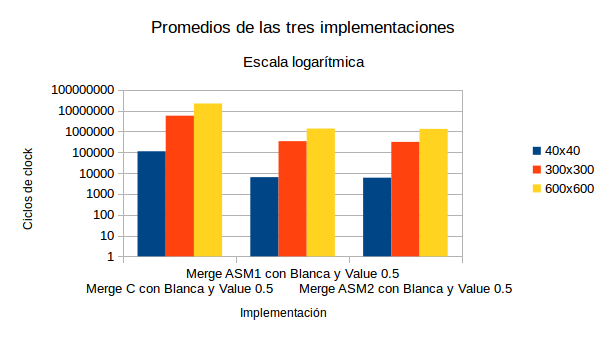
\includegraphics[width=90mm]{merge/grafico_merge_conBlancas.png}
%\caption{A simple caption \label{overflow}}
\end{figure}


\begin{tabular}{| l | l | l | l | l |}
\hline
Implementación & Color & 1600 píxeles & 90000 píxeles & 360000 píxeles\\
\hline
Merge C con Negra y Value 0.5 & azul & 112601.93 &	5639322.00 &	21469172.00\\ 
\hline
Merge C con Negra y Value 0.5 & blanco & 98544.67	& 5963986.00 &	21739485.33\\ 
\hline
Merge C con Negra y Value 0.5 & mixto & 111715.11	& 5427554.33 &	21890057.78\\ 
\hline
Merge C con Negra y Value 0.5 & negro & 121468.75	& 5994952.25 &	21164423.00\\
\hline
Merge C con Negra y Value 0.5 & rojo & 109971.00	& 5852953.63	& 21210556.00\\
\hline
Merge C con Negra y Value 0.5 & verde & 106222.00 &	5679551.50	& 20684177.00\\ 
\hline
Promedio & &  110087.24	& 5759719.95 &	21359645.19\\
\hline
Desvio estándard  && 7572.28	& 217719.09	& 436854.38\\
\hline
Porcentaje de desviación  && 6.88\%	& 3.78\% &	2.05\%\\
\hline
\end{tabular}


\begin{tabular}{| l | l | l | l | l |}
\hline
Implementación & Color & 1600 píxeles & 90000 píxeles & 360000 píxeles\\
\hline
Merge ASM1 con Negra y Value 0.5 & azul & 6670.00 &	339259.67 &	1370217.47\\ 
\hline
Merge ASM1 con Negra y Value 0.5 & blanco & 7953.00 &	335490.33	& 1379671.33\\ 
\hline
Merge ASM1 con Negra y Value 0.5 & mixto & 6369.33	& 341912.22 &	1356897.33\\ 
\hline
Merge ASM1 con Negra y Value 0.5 & negro & 6424.25 &	335257.00 &	1384766.75\\
\hline
Merge ASM1 con Negra y Value 0.5 & rojo & 7097.88 &	343915.63 &	1372561.50\\
\hline
Merge ASM1 con Negra y Value 0.5 & verde & 6359.50	& 345085.00 &	1389391.00\\ 
\hline
Promedio & &  6812.33	& 340153.31 &	1375584.23\\
\hline
Desvio estándard  && 625.27	& 4197.29	& 11651.52\\
\hline
Porcentaje de desviación  && 9.18\% &	1.23\% &	0.85\%\\
\hline
\end{tabular}


\begin{tabular}{| l | l | l | l | l |}
\hline
Implementación & Color & 1600 píxeles & 90000 píxeles & 360000 píxeles\\
\hline
Merge ASM2 con Negra y Value 0.5 & azul & 5993.67	& 309772.60 & 	1292696.93\\ 
\hline
Merge ASM2 con Negra y Value 0.5 & blanco & 6841.33	& 301941.67 &	1245065.00\\ 
\hline
Merge ASM2 con Negra y Value 0.5 & mixto & 6352.22	& 309041.00	& 1343273.56\\ 
\hline
Merge ASM2 con Negra y Value 0.5 & negro & 6628.00	& 320615.50	& 1338728.00\\
\hline
Merge ASM2 con Negra y Value 0.5 & rojo & 6009.38	& 305238.13	& 1357228.63\\
\hline
Merge ASM2 con Negra y Value 0.5 & verde & 6338.00	& 312857.75	& 1279955.25\\ 
\hline
Promedio & &  6360.43	& 309911.11	& 1309491.23\\
\hline
Desvio estándard  && 335.02	& 6471.35	& 43772.26\\
\hline
Porcentaje de desviación  && 5.27\% &	2.09\% &	3.34\%\\
\hline
\end{tabular}

\begin{tabular}{| l | l | l | l|}
\hline
Implementación  & 1600 píxeles & 90000 píxeles & 360000 píxeles\\
\hline
Merge C con Negra y Value 0.5  & 110087.24	5759719.95	21359645.19\\
\hline
Merge ASM1 con Negra y Value 0.5  & 6812.33	340153.31	1375584.23\\
\hline
Merge ASM2 con Negra y Value 0.5 & 6360.43	309911.11	1309491.23\\
\hline
\end{tabular}

\begin{figure}[ht]
\centering
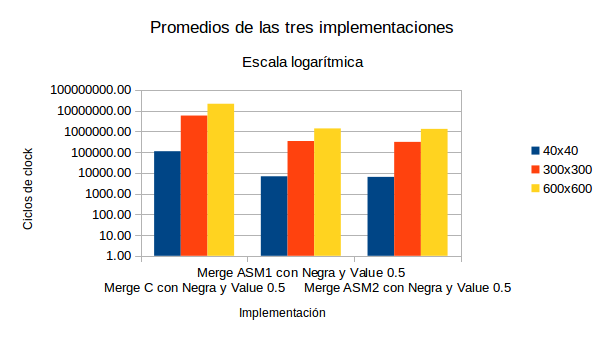
\includegraphics[width=90mm]{merge/grafico_merge_conNegras.png}
%\caption{A simple caption \label{overflow}}
\end{figure}
